\begin{frame}
\frametitle{Benchmarking DFT functionals}
\centering
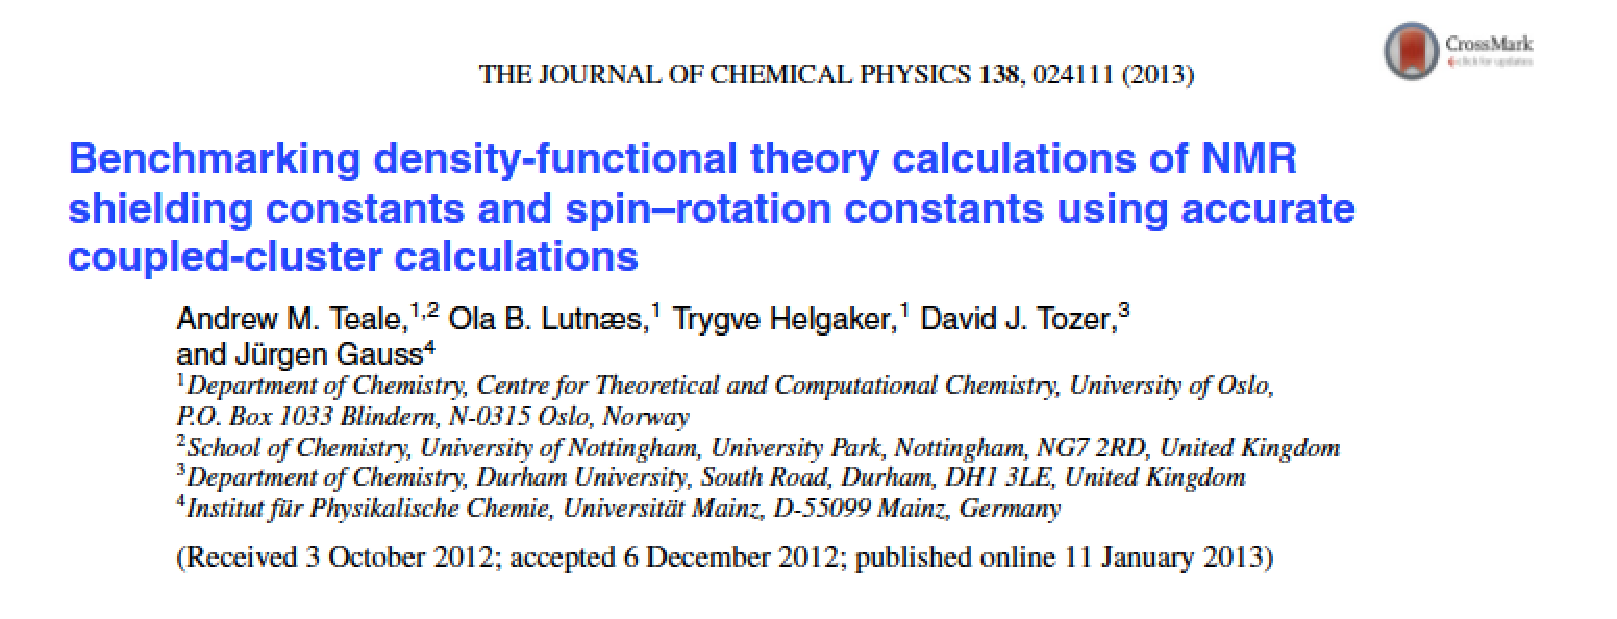
\includegraphics[scale=0.35]{figures/Teale_etal_2013.pdf}

\vspace{10mm}

\begin{columns}
\begin{column}[b]{0.5\textwidth}
    \textbf{Wave function methods}
    \begin{itemize}
        \item   RHF, CCSD, CCSD(T)
        \item   aug-cc-pCVXZ, X=D,T,Q
        \item   Basis set extrapolation
        \item   Comparison with experiment
    \end{itemize}
\end{column}
\begin{column}[b]{0.5\textwidth}
    \textbf{Density functional methods}
    \begin{itemize}
        \item   LDA, GGA, hybrid-GGA, OEP
        \item   aug-cc-pCVXZ, X=D,T,Q
        \item   Comparison with CCSD(T)
        \item   Comparison with experiment
    \end{itemize}
\end{column}
\end{columns}
\end{frame}

\begin{frame}
\frametitle{Benchmarking DFT functionals}

\vspace{13mm}

\centering
\textbf{Hartree-Fock extrapolation formula}
\begin{equation}
    \nonumber
    P_\infty = 
    \frac{P_X \exp{(\alpha X)} - P_Y \exp{(\alpha Y)}}
    {\exp{(\alpha X)} - \exp{(\alpha Y)}}
\end{equation}

\vspace{19mm}

\begin{columns}
\begin{column}[b]{0.5\textwidth}
    \textbf{Wave function methods}
    \begin{itemize}
        \item   RHF, CCSD, CCSD(T)
        \item   aug-cc-pCVXZ, X=D,T,Q
        \item   Basis set extrapolation
        \item   Comparison with experiment
    \end{itemize}
\end{column}
\begin{column}[b]{0.5\textwidth}
    \textbf{Density functional methods}
    \begin{itemize}
        \item   LDA, GGA, hybrid-GGA, OEP
        \item   aug-cc-pCVXZ, X=D,T,Q
        \item   Comparison with CCSD(T)
        \item   Comparison with experiment
    \end{itemize}
\end{column}
\end{columns}
\end{frame}

\begin{frame}
\frametitle{Benchmarking DFT functionals}

\centering
\textbf{Functionals}
\begin{multicols}{3}
\begin{itemize}
    \item Hartree-Fock
    \item LDA
    \item BLYP
    \item B3LYP
    \item PBE
    \item PBE0
\end{itemize}
\end{multicols}

\vspace{5mm}

\textbf{Molecules}
\begin{multicols}{4}
\begin{itemize}
    \item HF
    \item CO
    \item N$_2$
    \item H$_2$O
    \item HCN
    \item HOF
    \item O$_3$
    \item NH$_3$      
    \item CH$_2$O     
    \item CH$_4$      
    \item C$_2$H$_4$  
    \item AlF         
    \item CH$_3$F     
    \item C$_3$H$_4$  
    \item FCCH        
    \item FCN         
    \item H$_2$S      
    \item HCP         
    \item HFCO        
    \item H$_2$C$_2$O 
    \item LiF         
    \item LiH        
    \item N$_2$O     
    \item OCS        
    \item OF$_2$     
    \item H$_4$C$_2$O
    \item PN         
    \item SO$_2$     
\end{itemize}
\end{multicols}
\end{frame}

\begin{frame}
\frametitle{Comparison with Complete Basis Set limit}
\textbf{MW calculations}
\begin{itemize}
    \item   MRChem
    \item   MWX: $\epsilon=10^{-X}, X=3,4,5,6$
\end{itemize}

\vspace{5mm}

\textbf{GTO calculations}
\begin{itemize}
    \item   Teale \etal
    \item   XZ: aug-cc-pCVXZ, X = T,Q
    \item   $[$TQ$\alpha]$: Extrapolated aug-cc-pCV$[$TQ$]$Z with exponential
            parameter $\alpha$
\end{itemize}

\vspace{5mm}

\textbf{Error analysis}
\begin{itemize}
    \item   NMR shielding constant (ppm)
    \item   Average over all 28 molecules
    \item   MW6 is taken as CSB reference
\end{itemize}
\end{frame}

\begin{frame}
\frametitle{Comparison with Complete Basis Set limit}
\centering
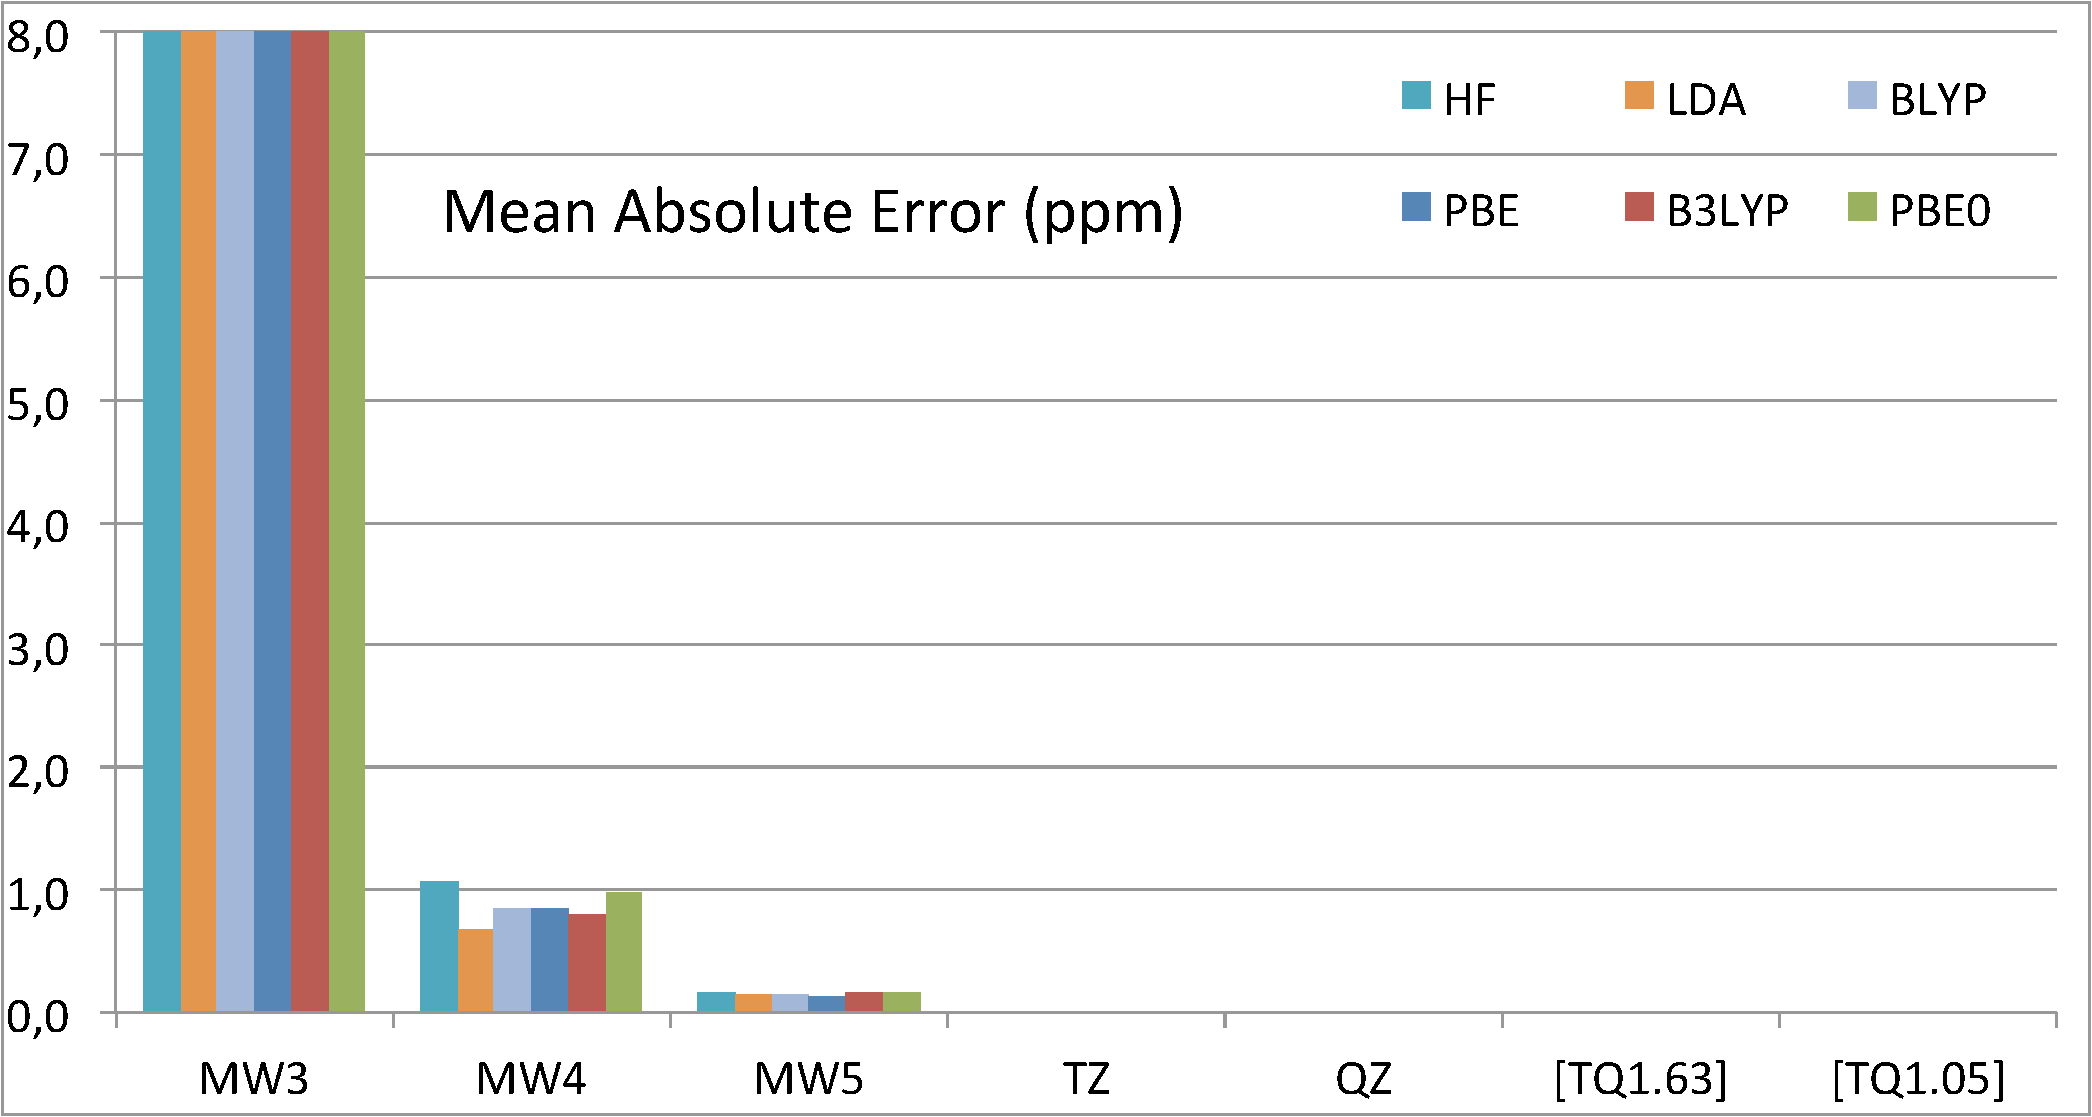
\includegraphics[scale=0.3]{figures/mae_bas_1.pdf}
\end{frame}

\begin{frame}
\frametitle{Comparison with Complete Basis Set limit}
\centering
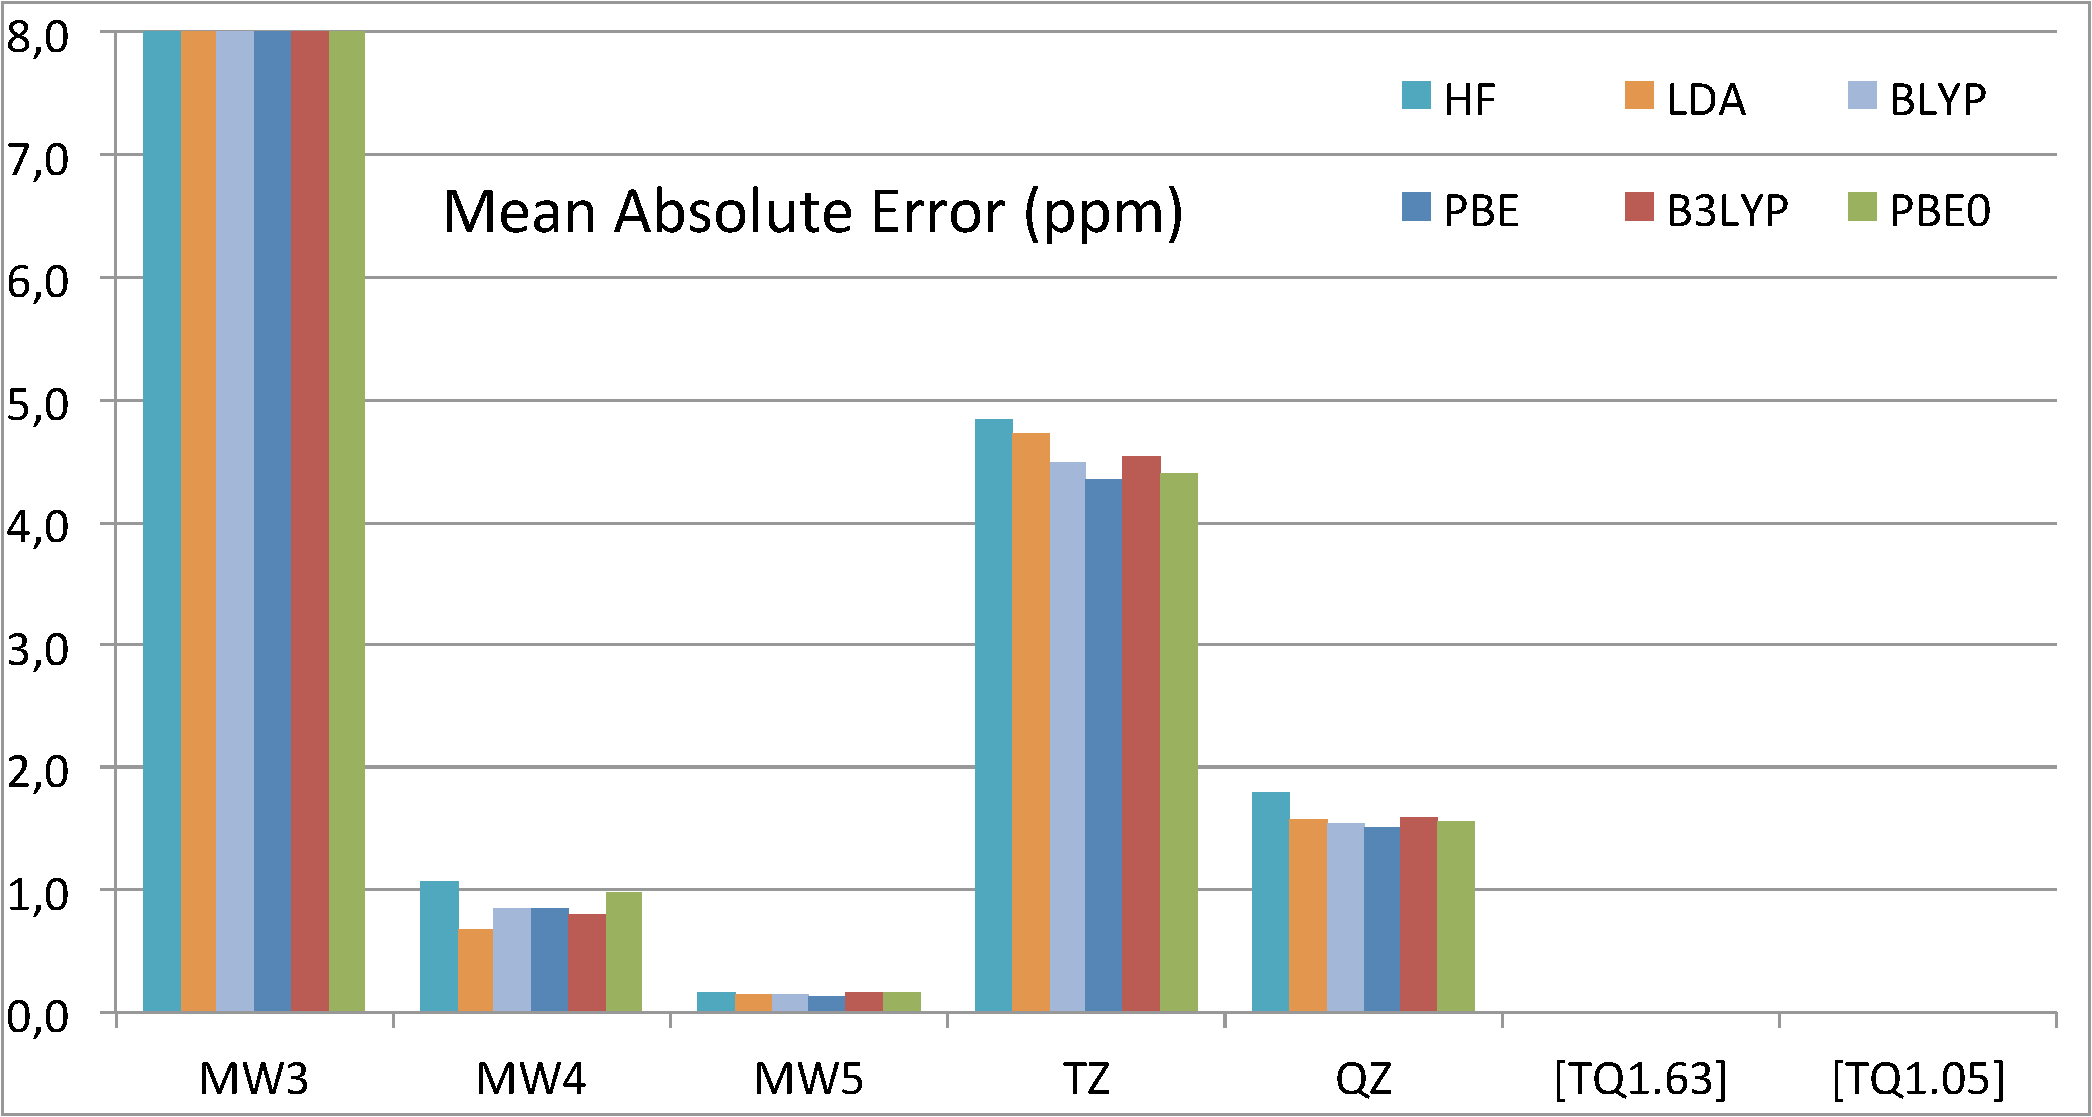
\includegraphics[scale=0.3]{figures/mae_bas_2.pdf}
\end{frame}

\begin{frame}
\frametitle{Comparison with Complete Basis Set limit}
\centering
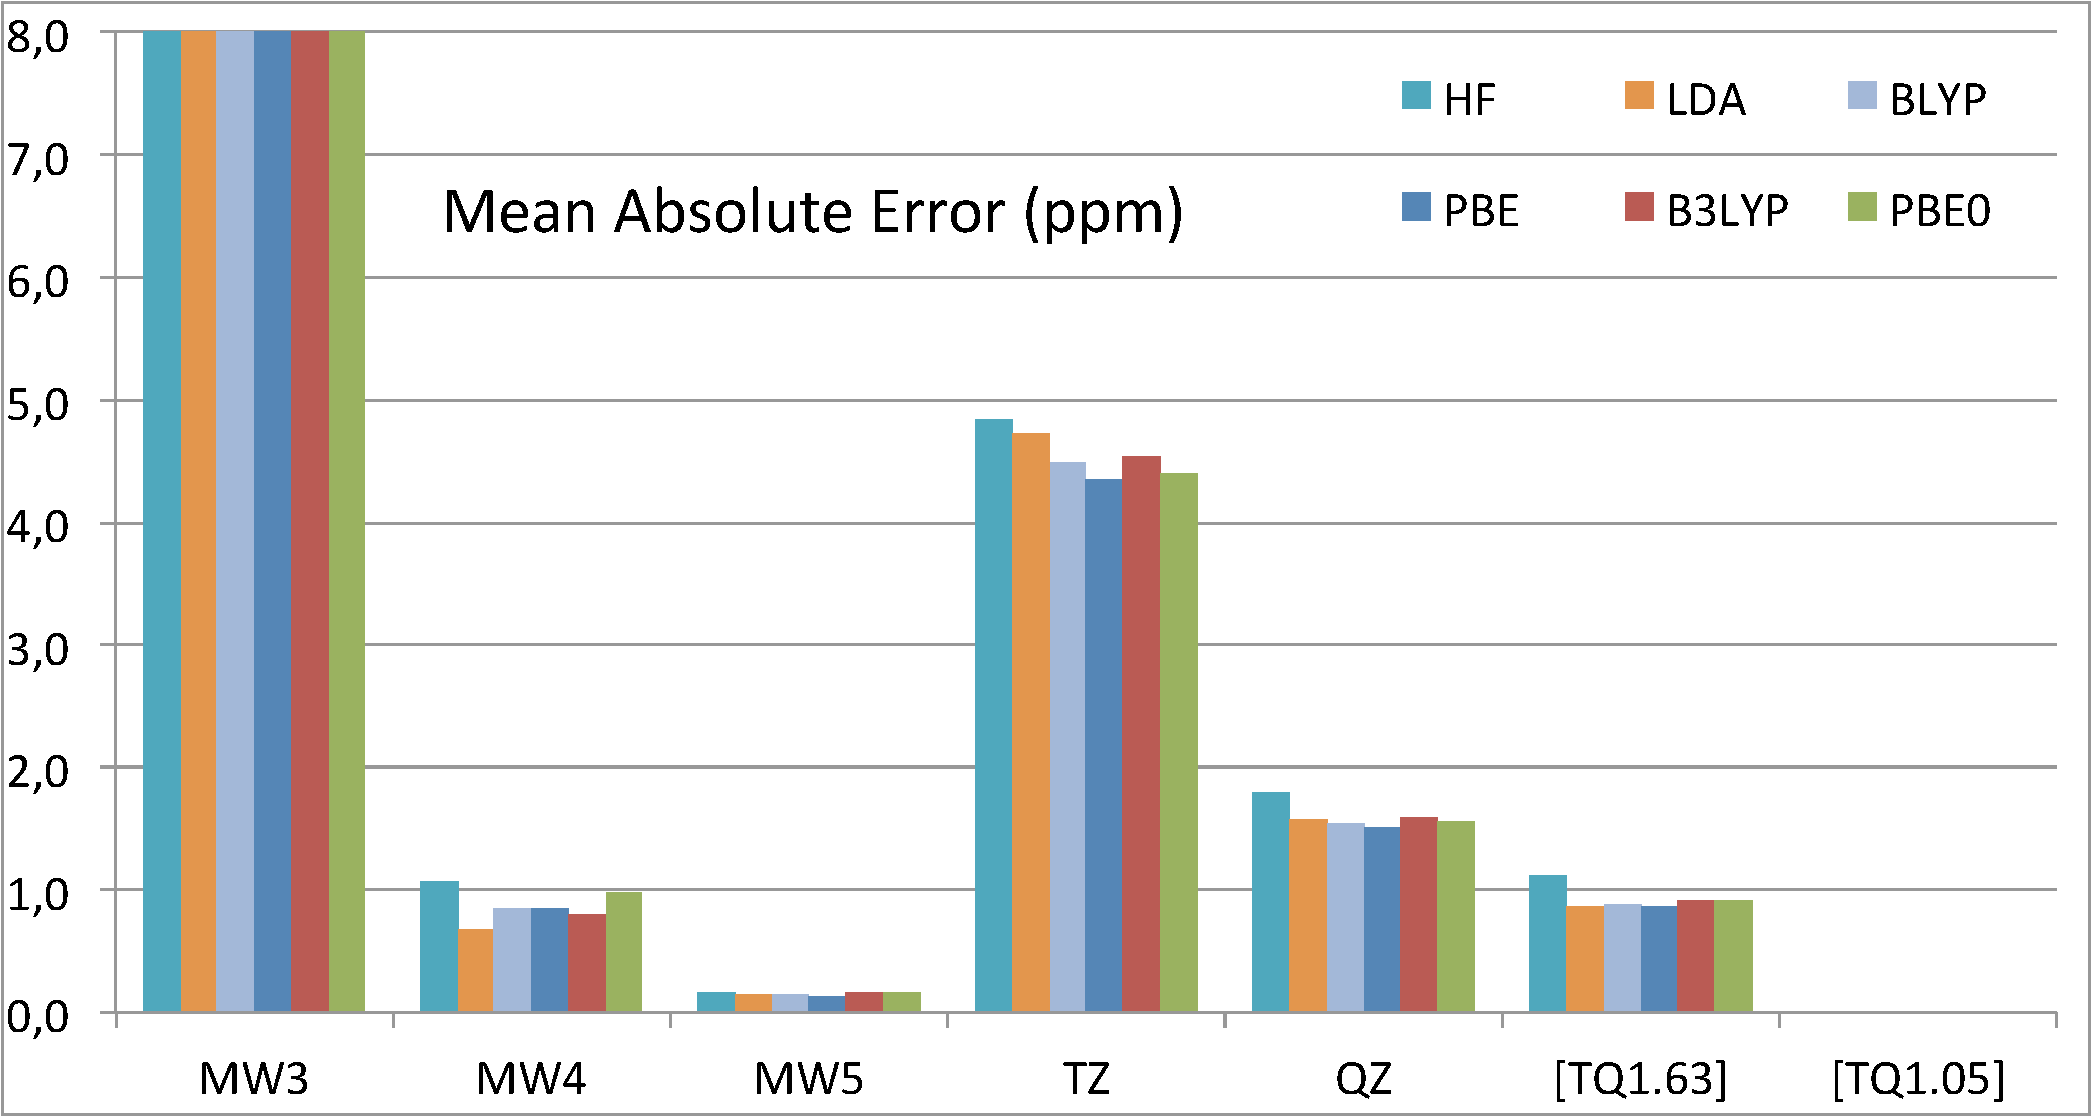
\includegraphics[scale=0.3]{figures/mae_bas_3.pdf}
\end{frame}

\begin{frame}
\frametitle{Comparison with Complete Basis Set limit}
\centering
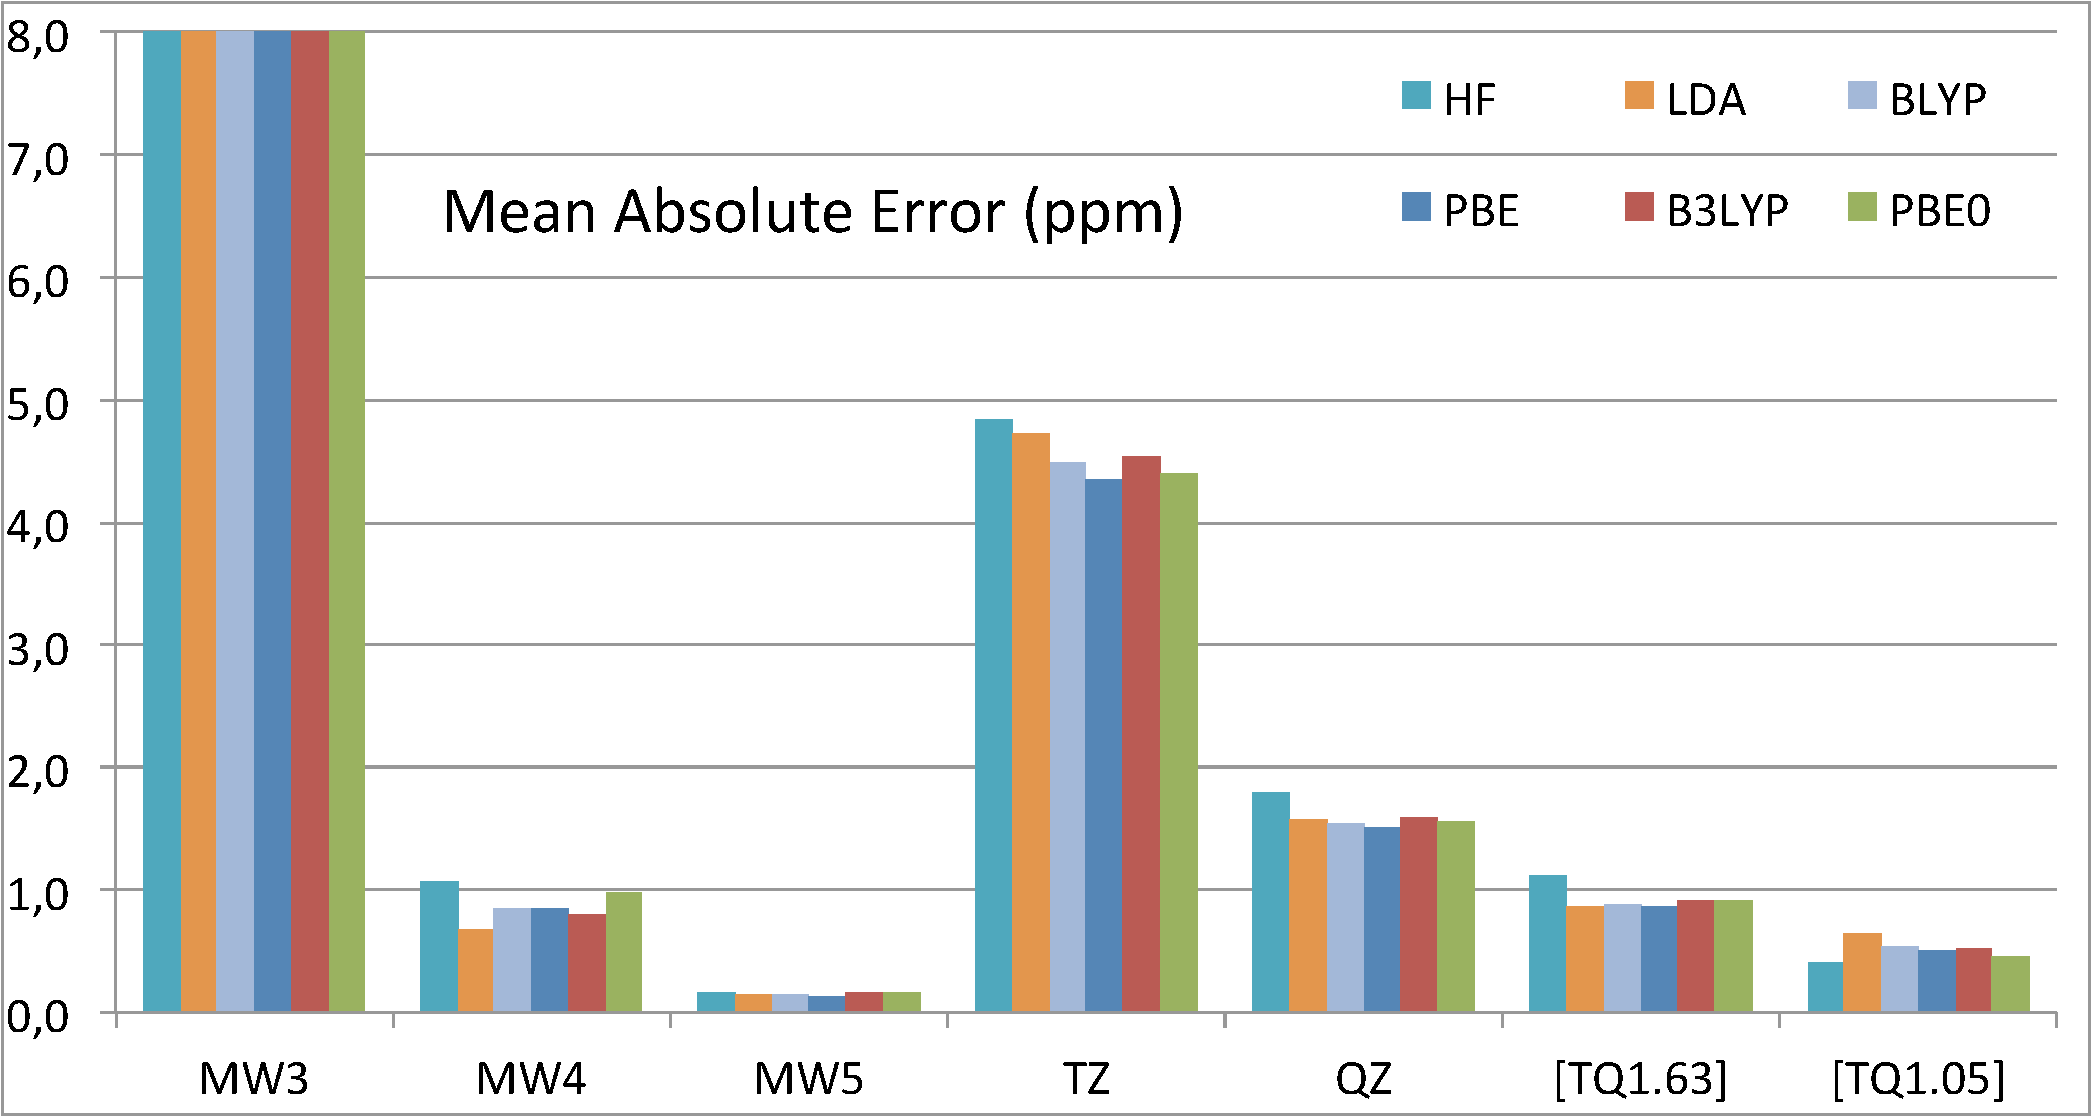
\includegraphics[scale=0.3]{figures/mae_bas_4.pdf}
\end{frame}

\begin{frame}
\frametitle{Computation time}
\textbf{MW calculations}
\begin{itemize}
    \item   MRChem
    \item   16/20 CPUs on Stallo
    \item   MWX: $\epsilon=10^{-X}, X=3,4,5,6$
\end{itemize}

\vspace{5mm}

\textbf{GTO calculations}
\begin{itemize}
    \item   Dalton
    \item   1 CPU on Stallo
    \item   XZ: aug-cc-pCVXZ, X = T,Q
\end{itemize}

\vspace{5mm}

\textbf{Timings}
\begin{itemize}
    \item   Average over all 28 molecules
    \item   4 SCF optimizations (ground-state + 3 response)
    \item   Minutes wall-time on 16 CPUs (renormalized)
\end{itemize}
\end{frame}

\begin{frame}
\frametitle{Computation time}
\centering
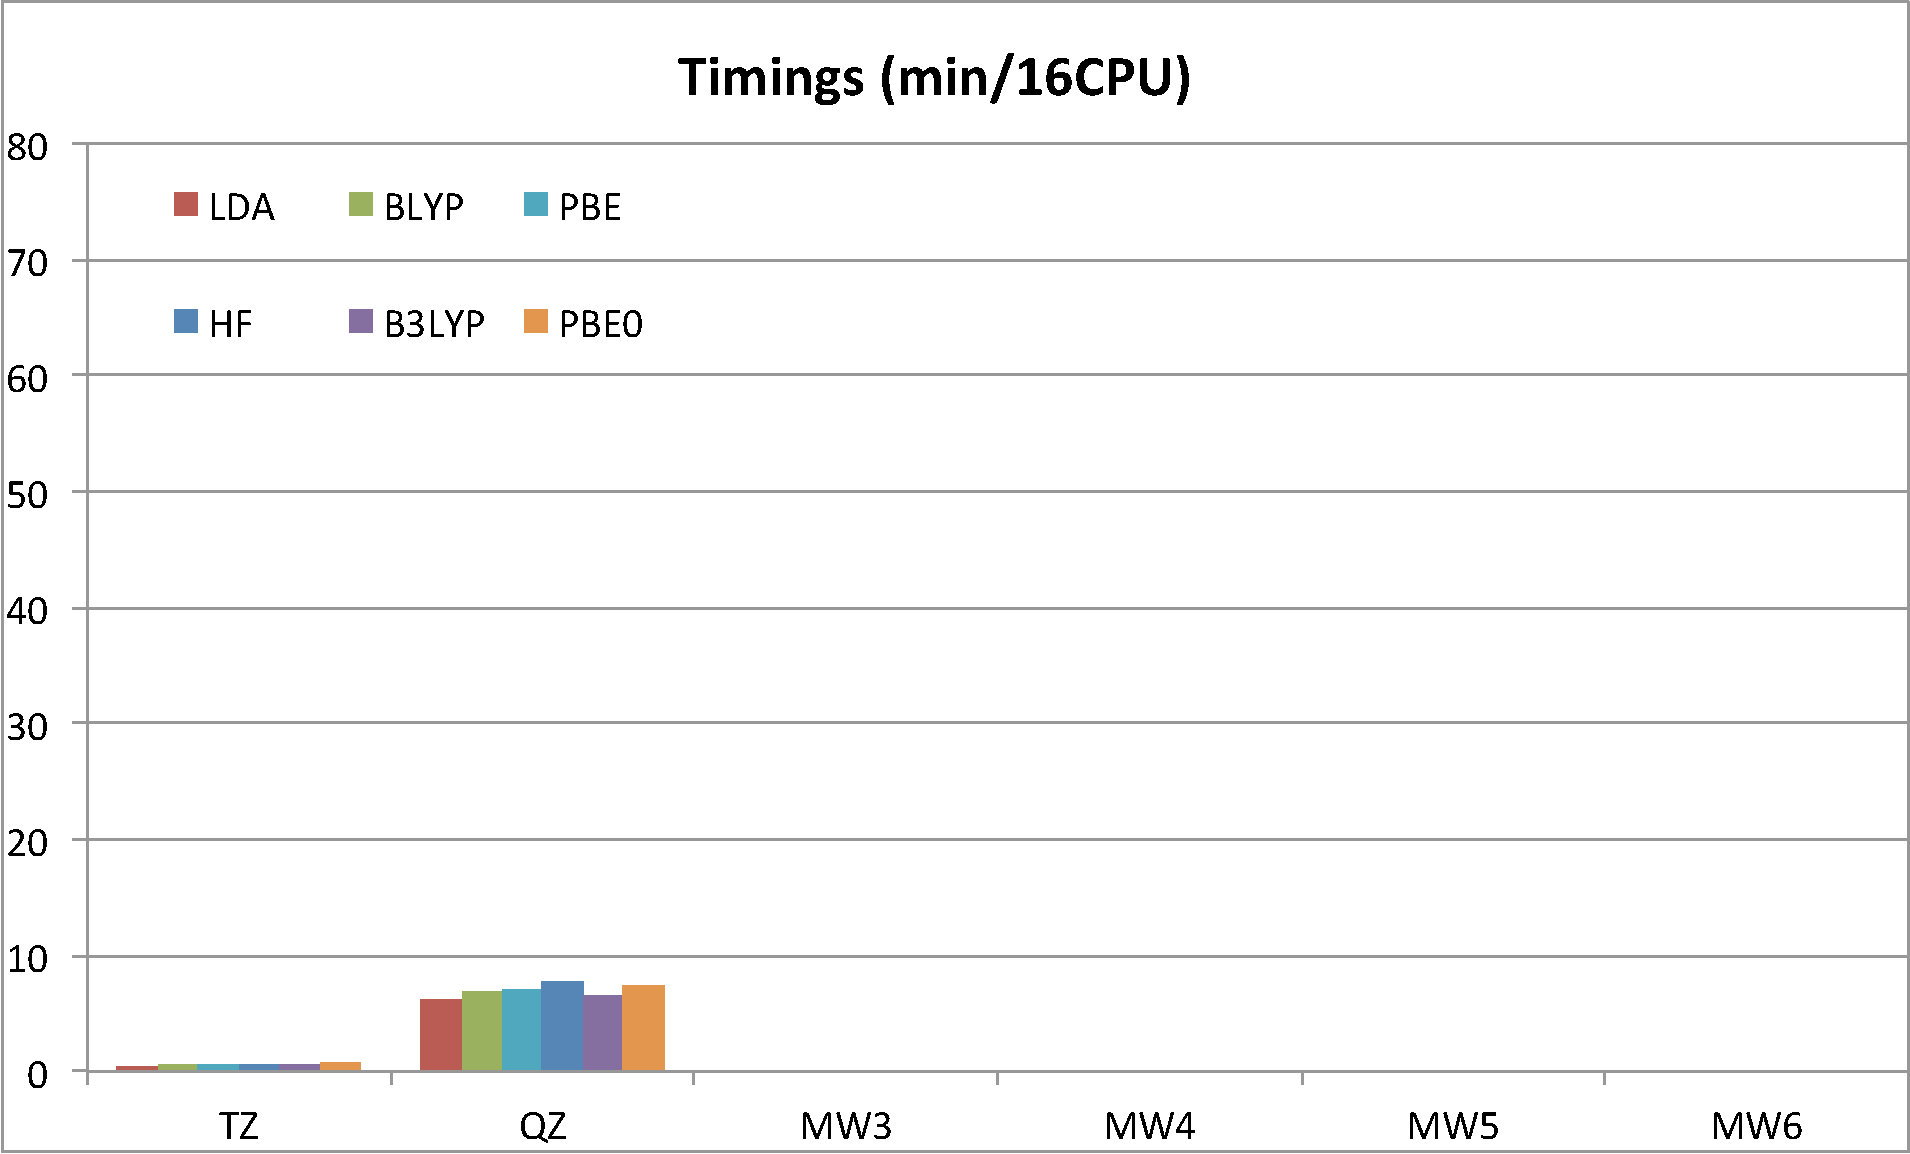
\includegraphics[scale=0.3]{figures/time_1.pdf}
\end{frame}

\begin{frame}
\frametitle{Computation time}
\centering
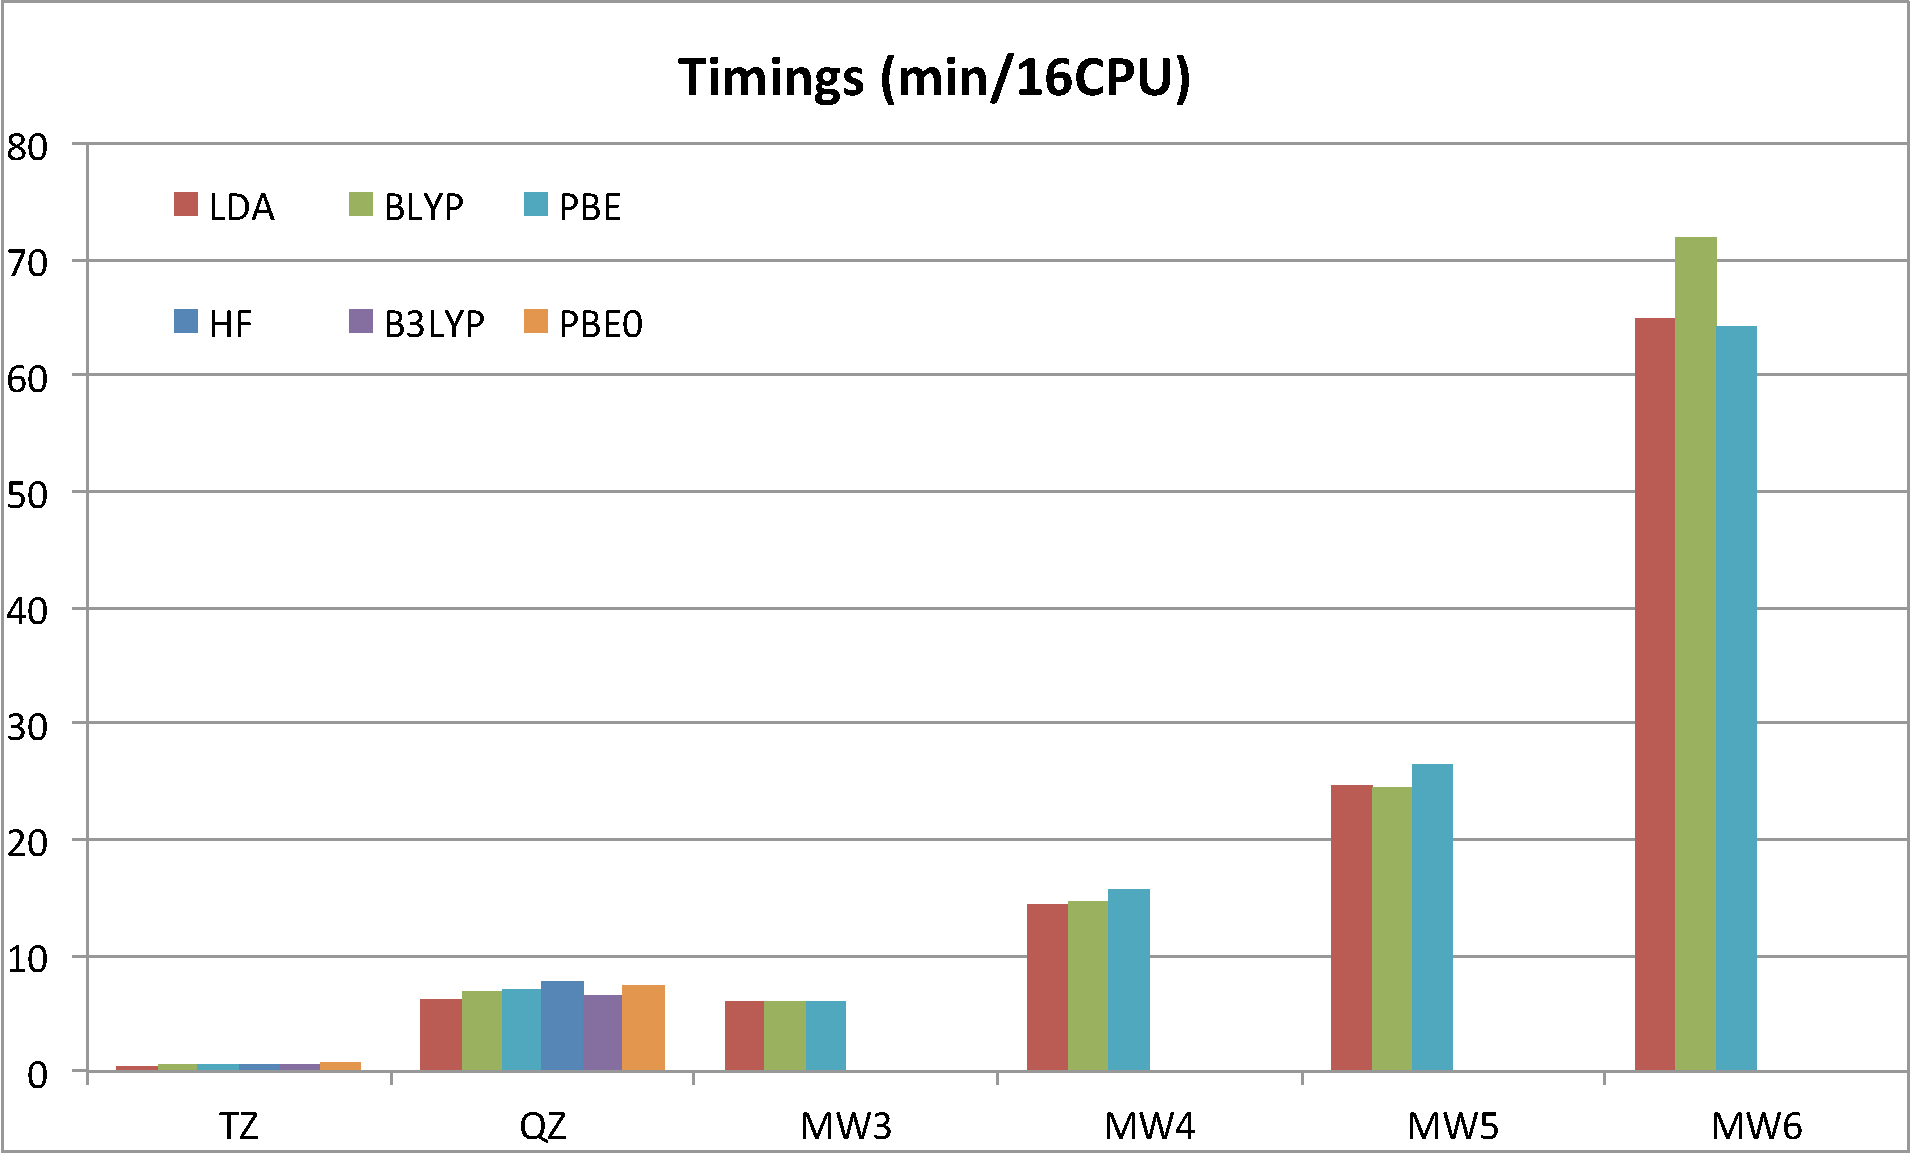
\includegraphics[scale=0.3]{figures/time_2.pdf}
\end{frame}

\begin{frame}
\frametitle{Computation time}
\centering
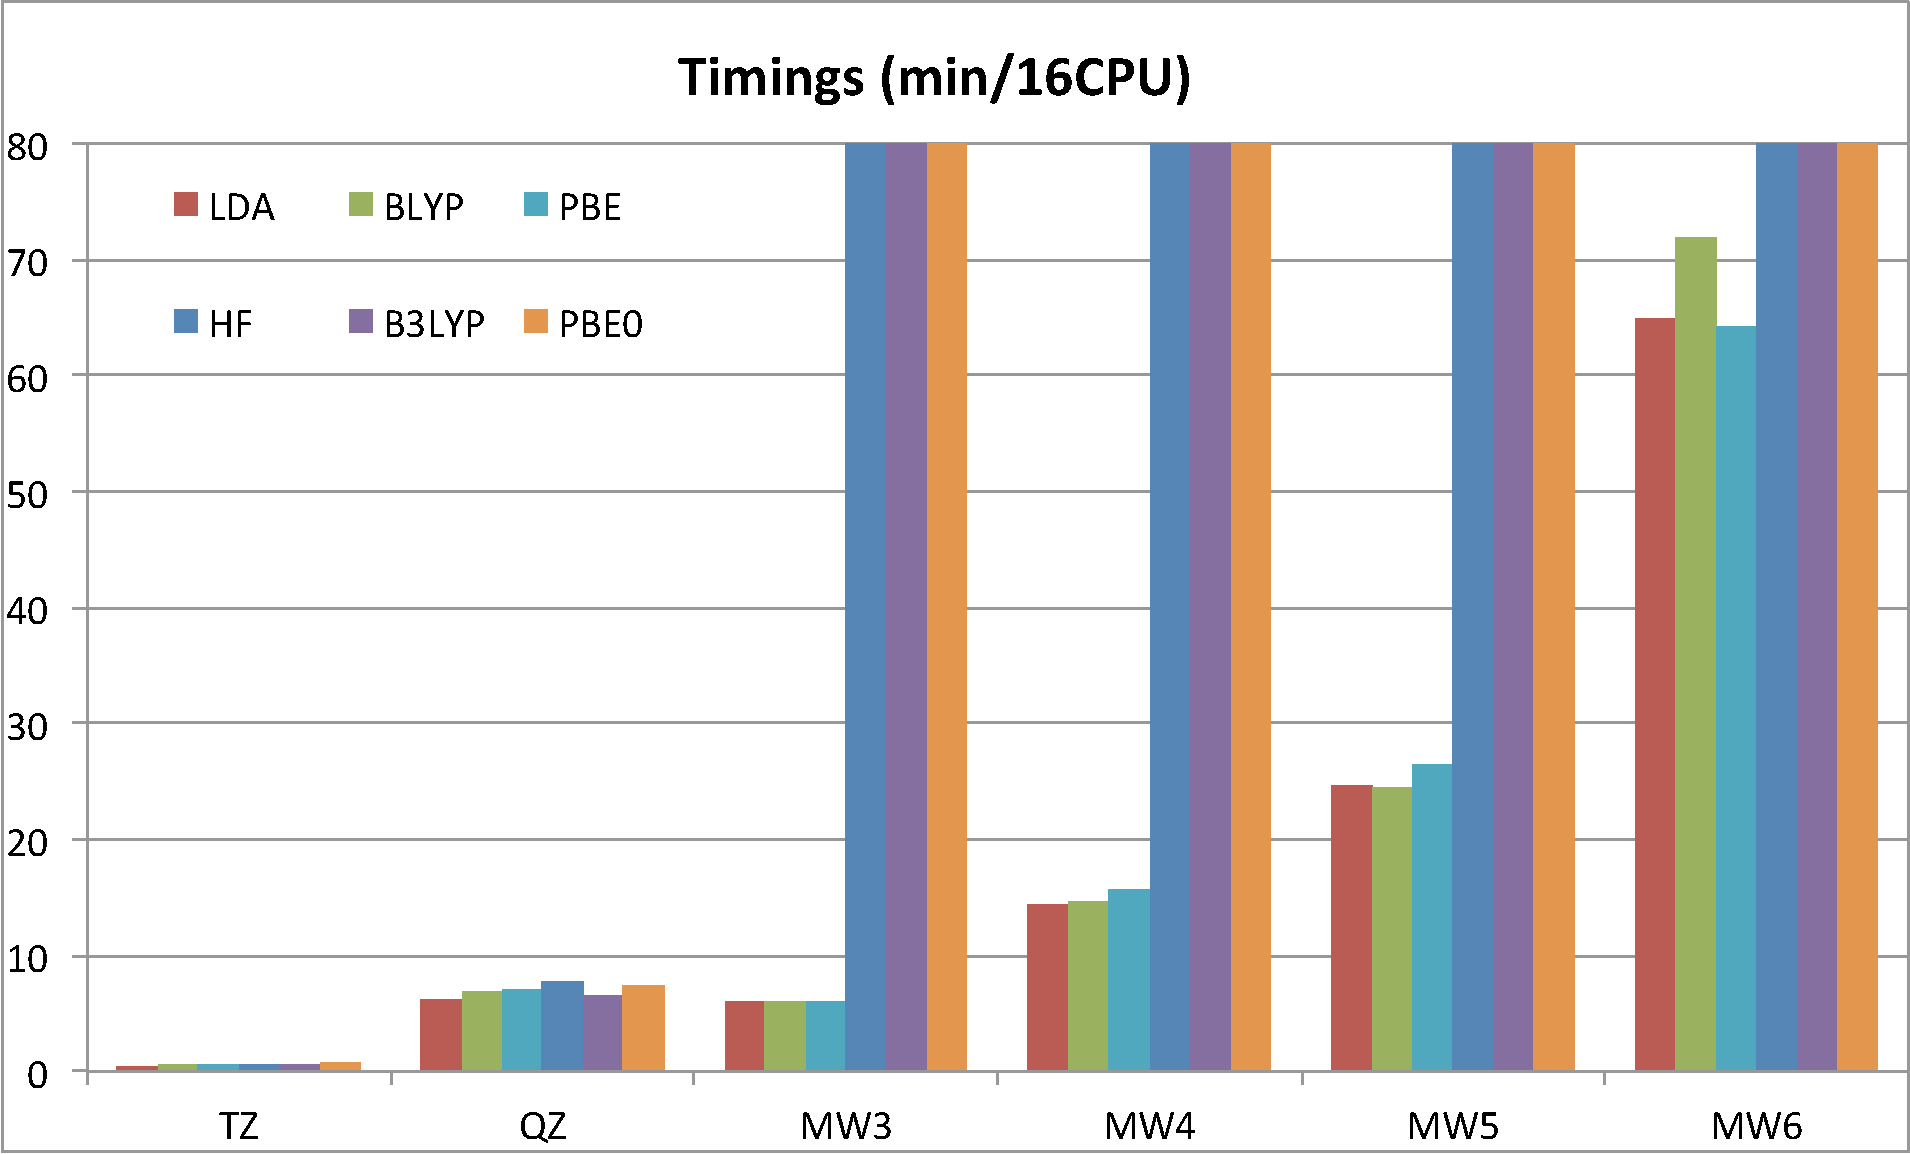
\includegraphics[scale=0.3]{figures/time_3.pdf}
\end{frame}

\begin{frame}
\frametitle{Computation time}
\centering
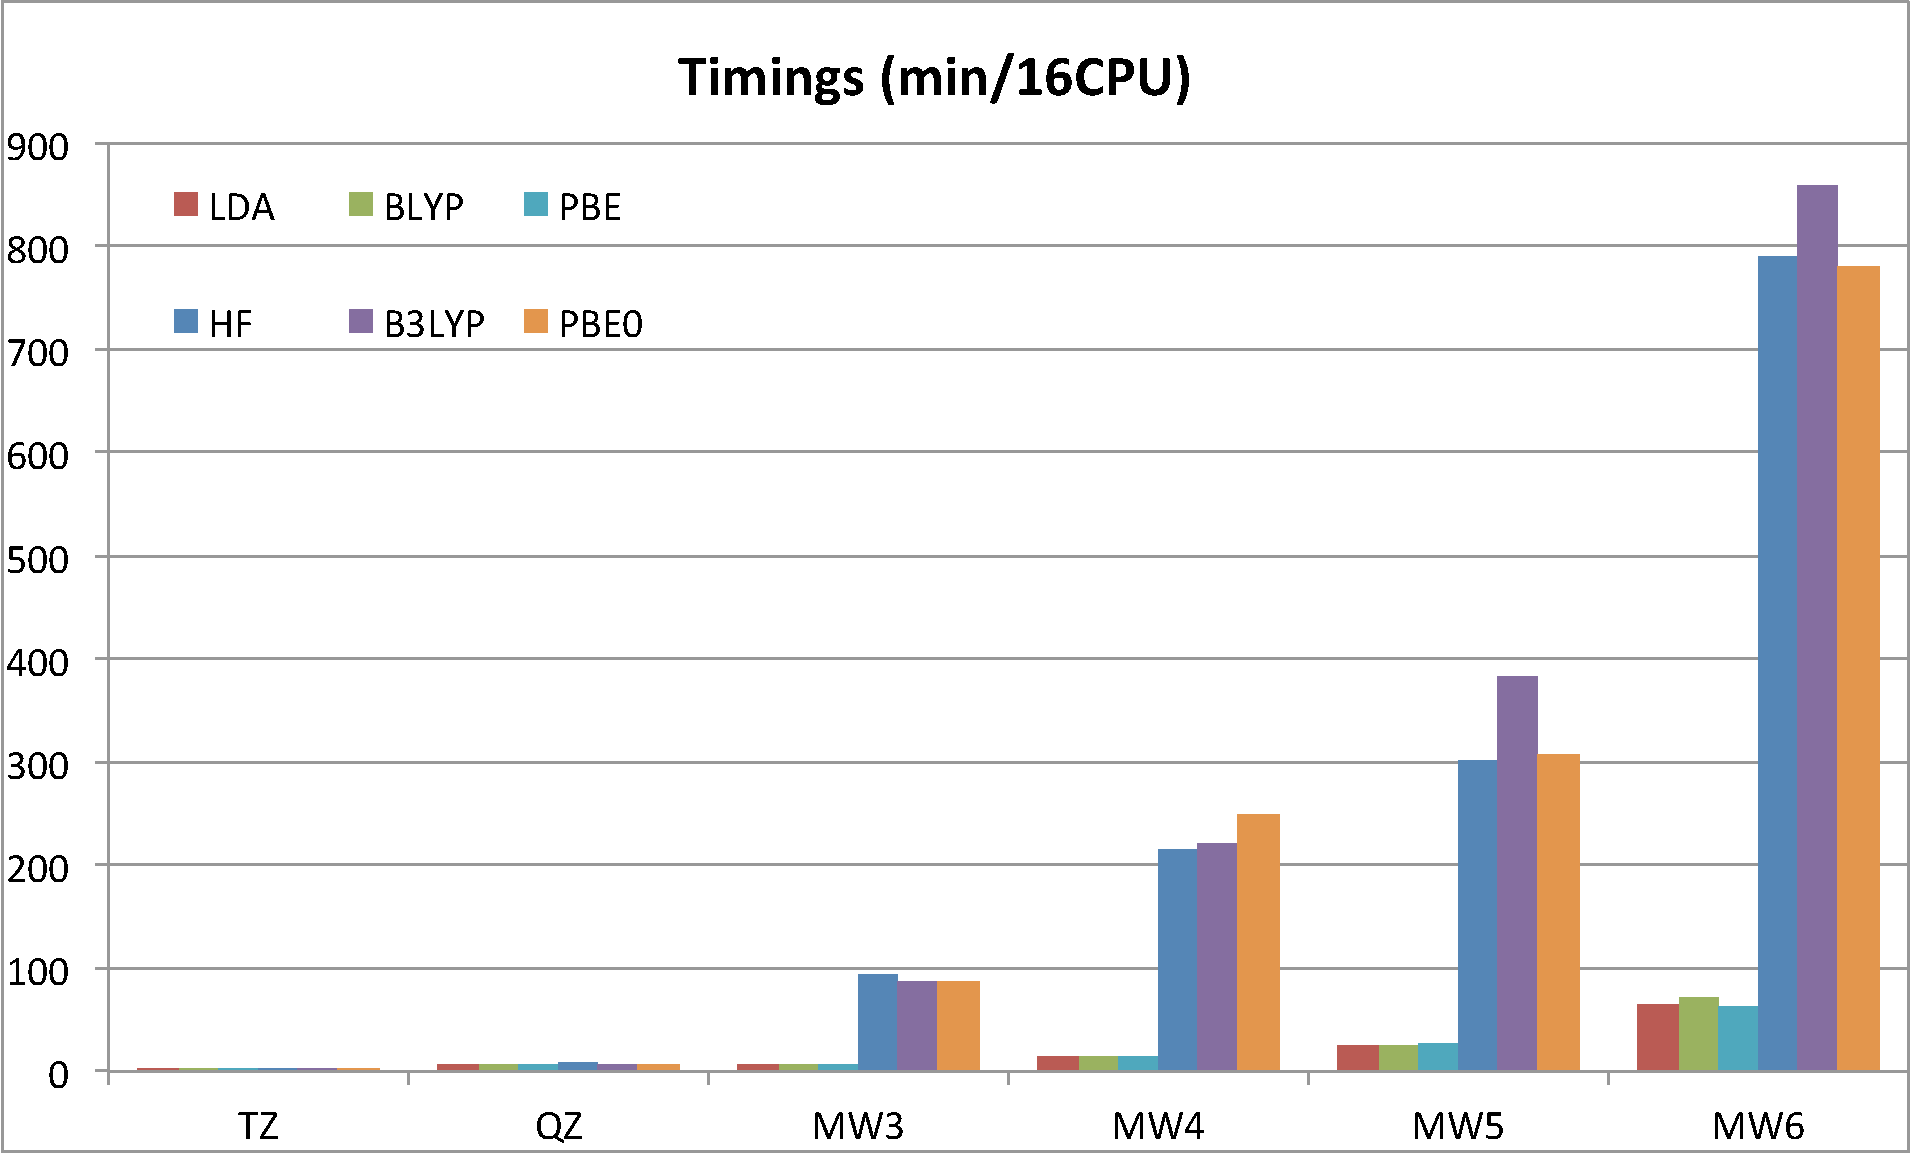
\includegraphics[scale=0.3]{figures/time_4.pdf}
\end{frame}

\begin{frame}
\frametitle{Comparison with Experiment}
\textbf{Calculations}
\begin{itemize}
    \item   MW calculations by MRChem
    \item   GTO calculations from Teale \etal
    \item   Basis sets: DZ, TZ, QZ, MW6
\end{itemize}

\vspace{10mm}

\textbf{Error analysis}
\begin{itemize}
    \item   NMR shielding constant (ppm)
    \item   1/4 of the data set excluded
    \item   Empirical equilibrium (experiments including ZPVC) is taken as reference
\end{itemize}
\end{frame}


\begin{frame}
\frametitle{Comparison with Experiment}
\centering
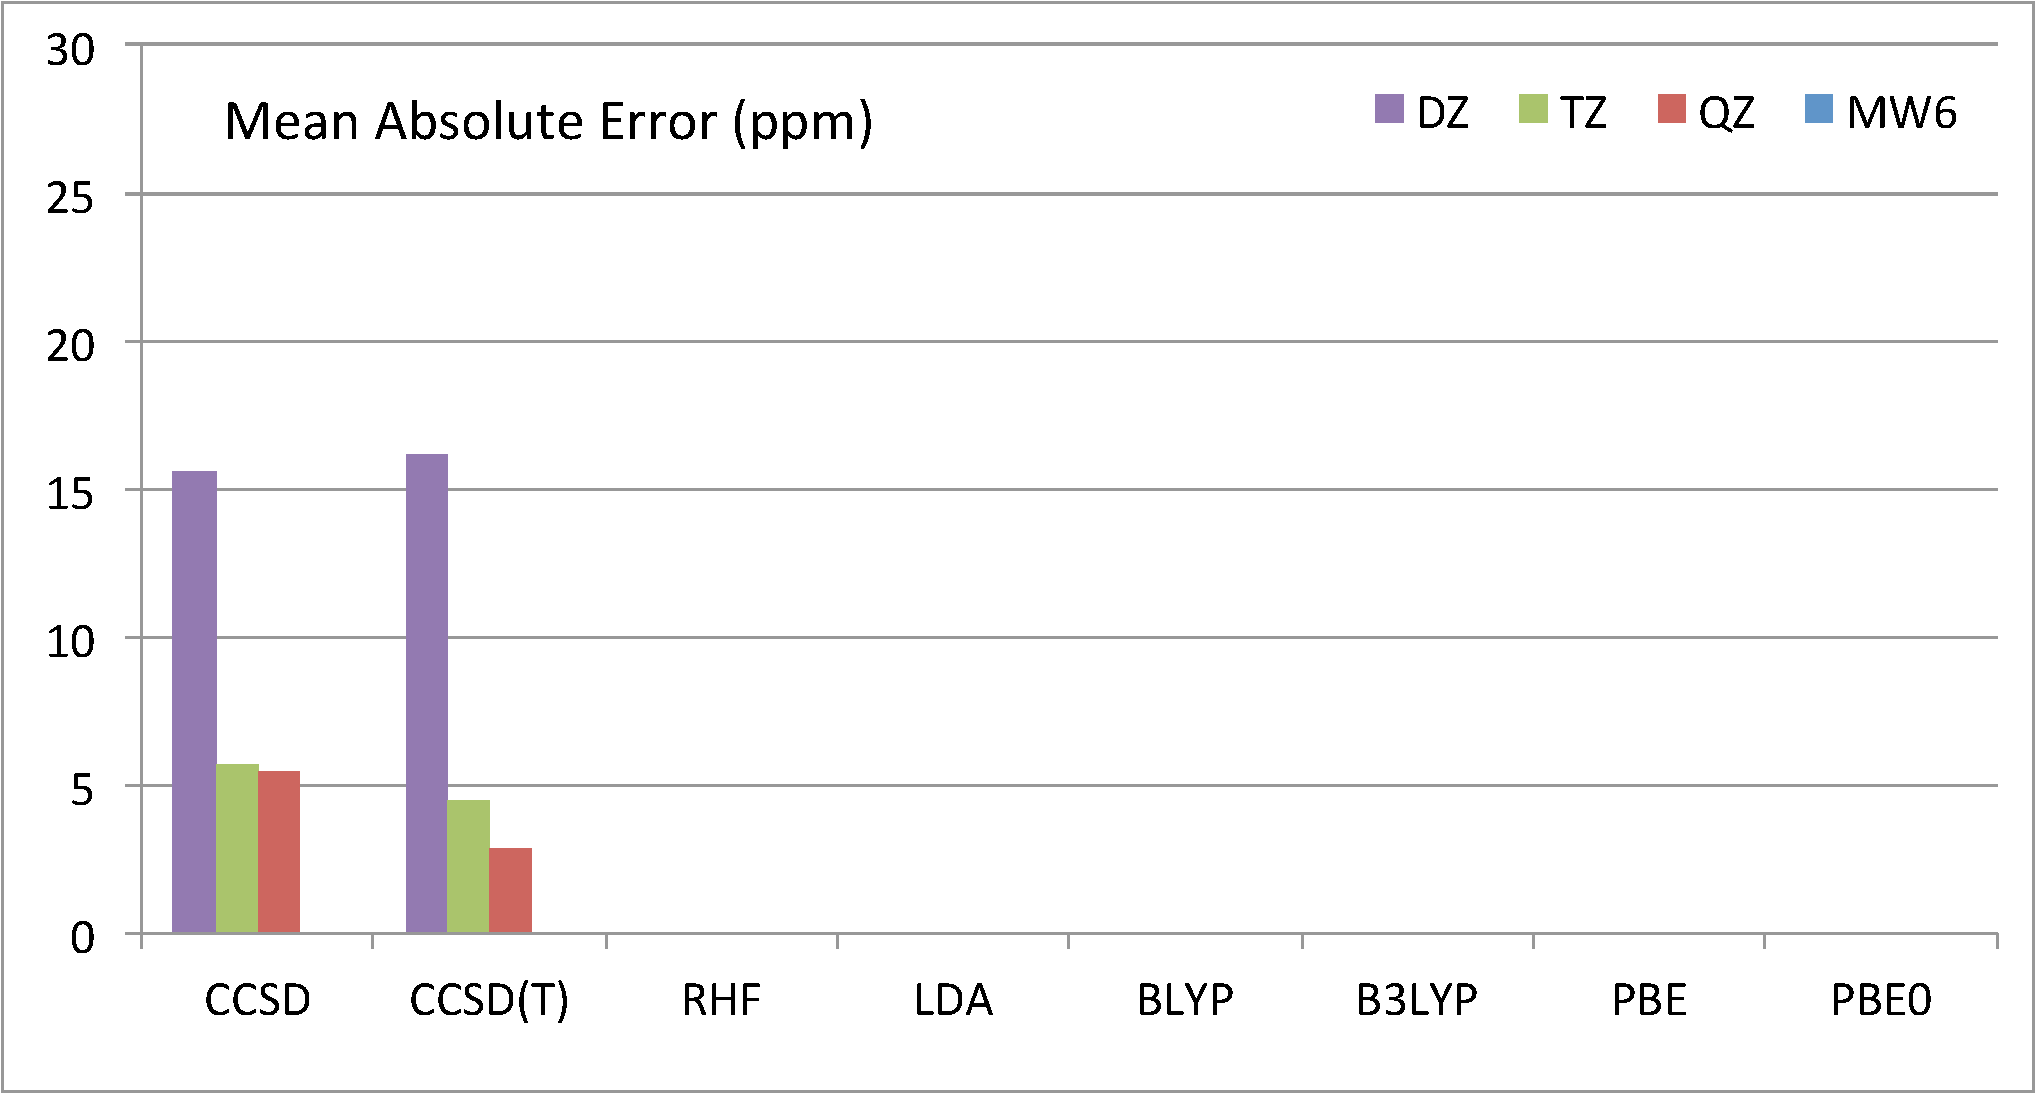
\includegraphics[scale=0.3]{figures/mae_exp_1.pdf}
\end{frame}

\begin{frame}
\frametitle{Comparison with Experiment}
\centering
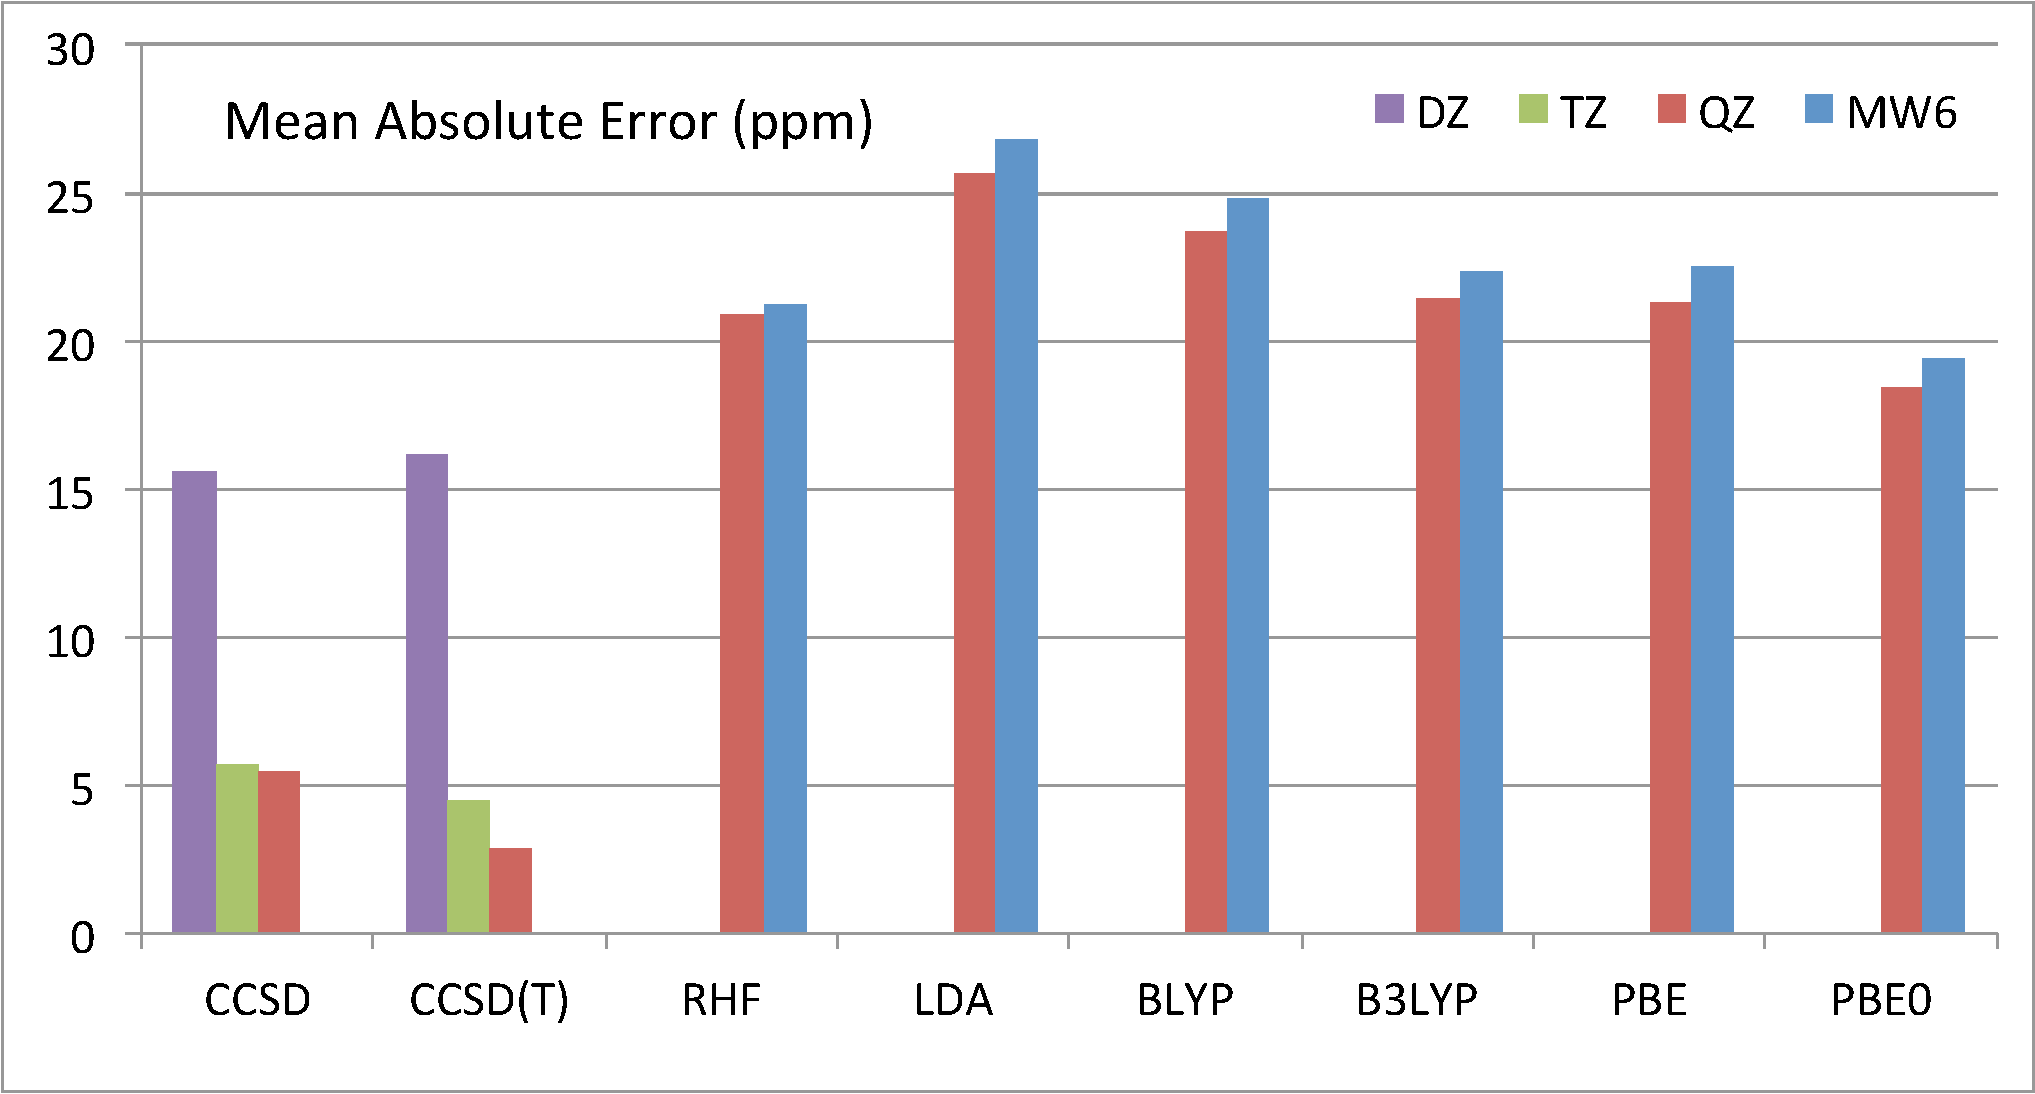
\includegraphics[scale=0.3]{figures/mae_exp_2.pdf}
\end{frame}

\begin{frame}
\frametitle{Comparison with Experiment}
\centering
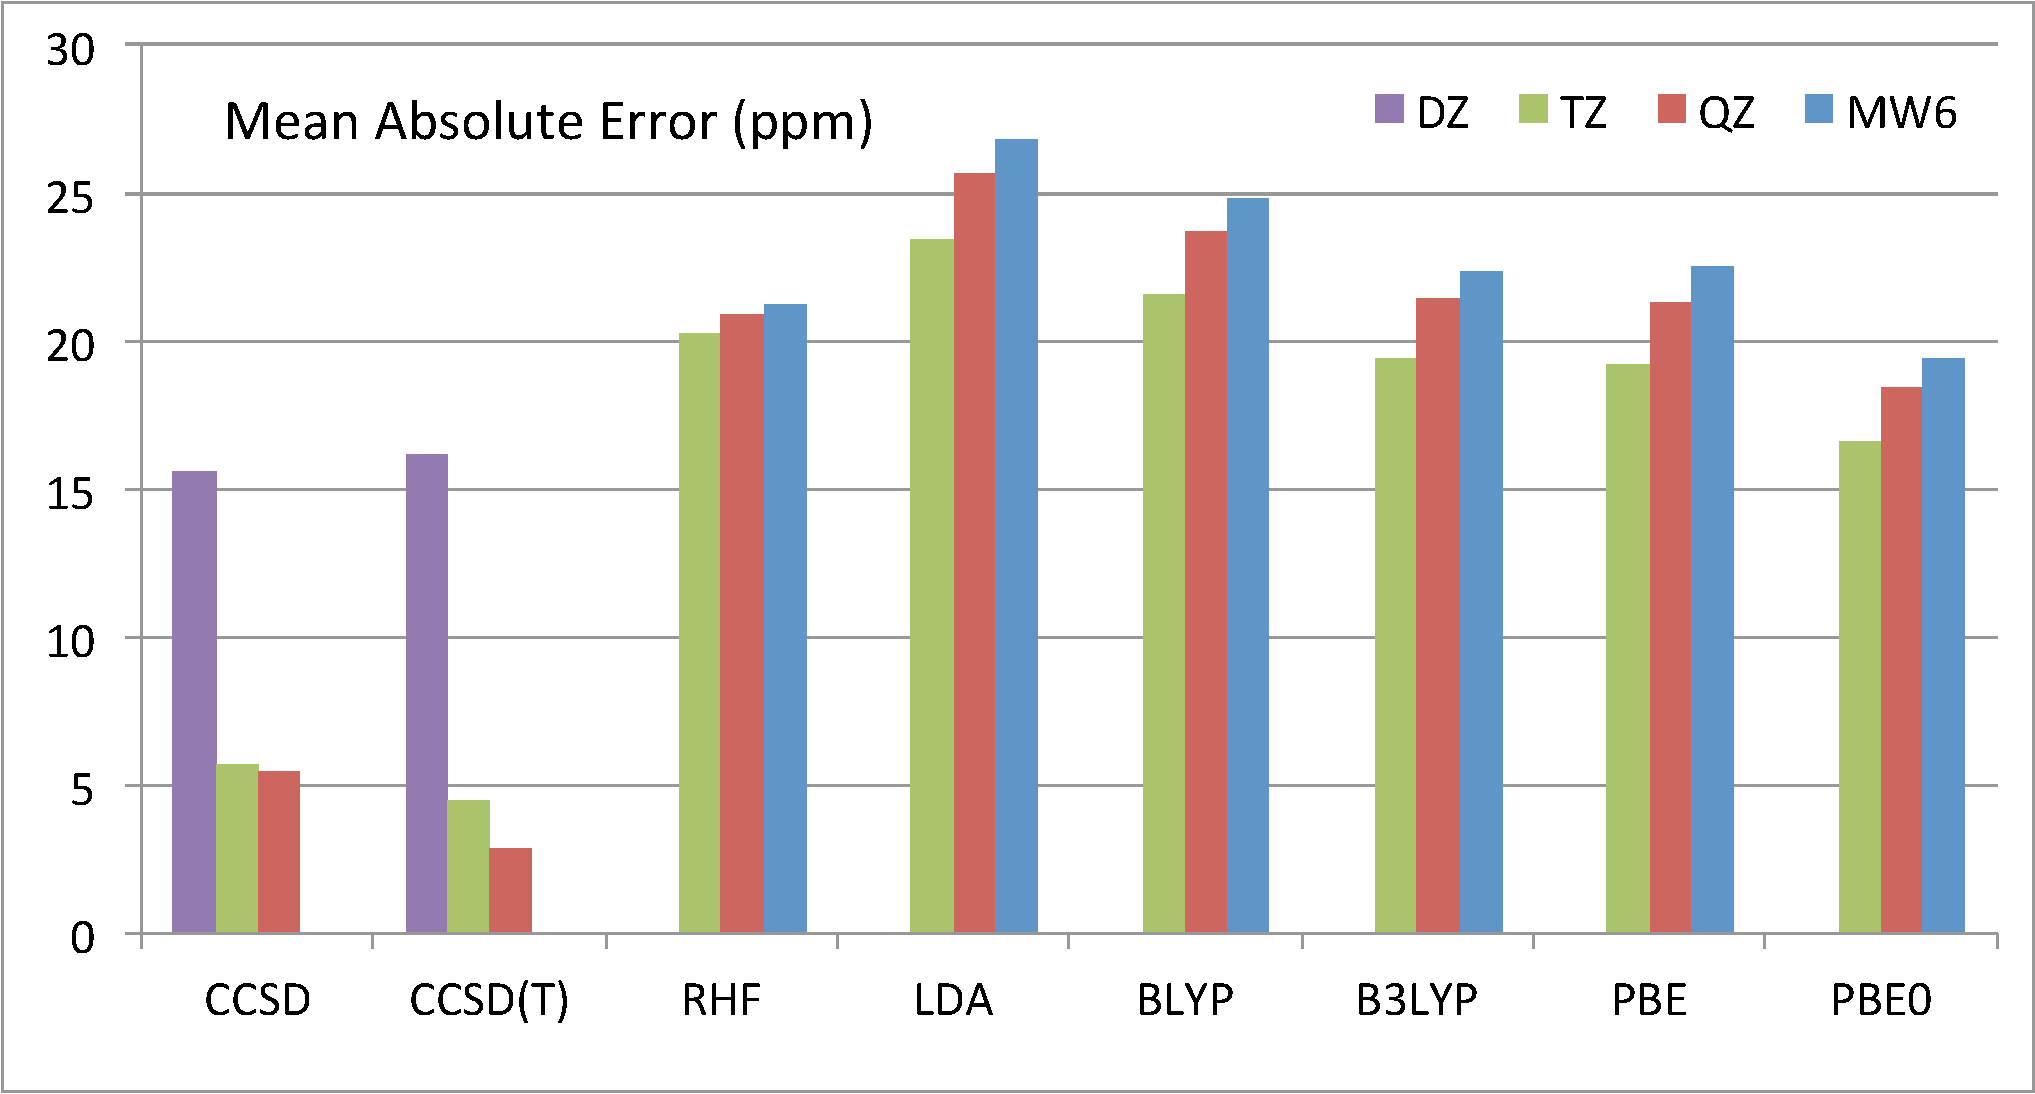
\includegraphics[scale=0.3]{figures/mae_exp_3.pdf}
\end{frame}

\begin{frame}
\frametitle{Comparison with Experiment}
\centering
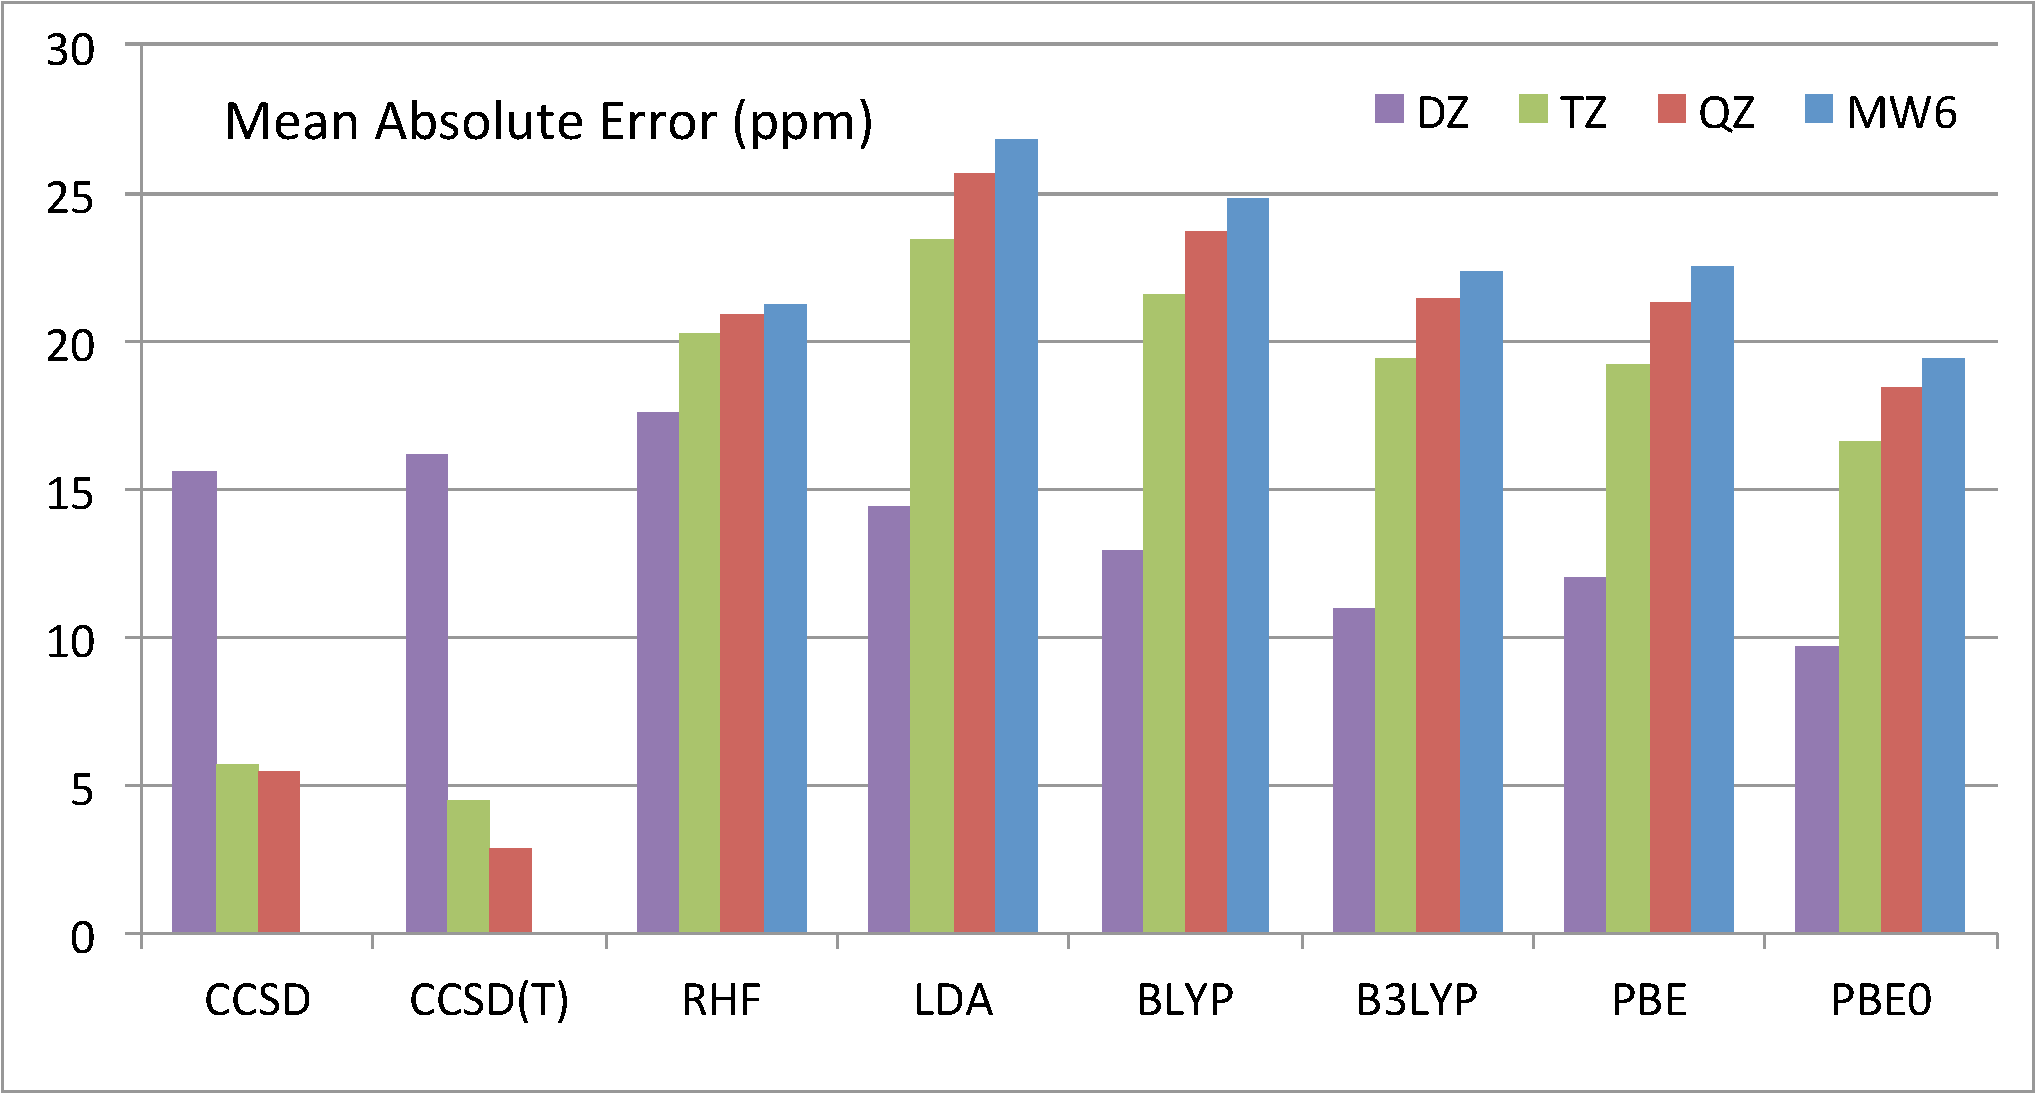
\includegraphics[scale=0.3]{figures/mae_exp_4.pdf}
\end{frame}
